\documentclass[english]{article}
\usepackage[T1]{fontenc}
\usepackage[latin9]{inputenc}
\usepackage{babel}
\usepackage{graphicx}
\begin{document}
\title{BSC-ROBOTMOTION second stage plan}\author{David Churchill, Supervisor: Charles Fox}\date{2019-11-01 12:28}\maketitle
\begin{center}


\includegraphics[width=6cm]{/home/charles/git/pandagantt/example_input//logo1.png}


\includegraphics[width=6cm]{/home/charles/git/pandagantt/example_input//logo2.png}


\includegraphics[width=6cm]{/home/charles/git/pandagantt/example_input//logo3.png}

\end{center}

\newpage

\section{Project overview}

Mobile robotics research on new AI planning algorithms is dependent on a lower level technology stack include physical and simulated vehicles, motor controllers, and motion controllers. A motion controller takes as its input a short-term desired trajectory for the robot, such as a curved path over a few meters and a few seconds, and outputs desired wheel speeds over real time to implement this trajectory. This project implements a simulation and a motion controller for a real Lincoln research robot, for use in real Lincoln robotics research. It has two main parts. First, a simulation will be developed in Gazebo to accurately reproduce the physics of a real Lincoln robot, including simulation of its masses, motor controllers, and frictions. Second, the simulation will be used to port Lincoln’s standard motion control stack (based on movebase with timed elastic bands) for use on the new robot. Once ported, the stack will be tested in simulation and optionally on the real robot. The final deliverable is the ability for a user to input a desired destination pose and have the system drive the robot to it from its start pose, for short distance trajectories with no obstacles.\newpage

\section{Work package overview}

\subsection*{WP1: Simulation}

Objectives: Create 3D simulation of robot.

Description: Shall be developed in Gazebo robotics simulator. Shall include experiments measuring properties of the physical vehicle to ensure accurate simulation. Attention shall be paid to wheel friction in particular.

\subsection*{WP2: Motion control}

Objectives: Port Lincoln's movebase stack to the simulated robot.

Description: The simulation shall be used to port Lincoln’s standard motion
control stack (based on movebase with timed elastic bands) for use
on the new robot. Once ported, the stack will be tested in simulation
and optionally on the real robot



\newpage

\section{Gantt chart}

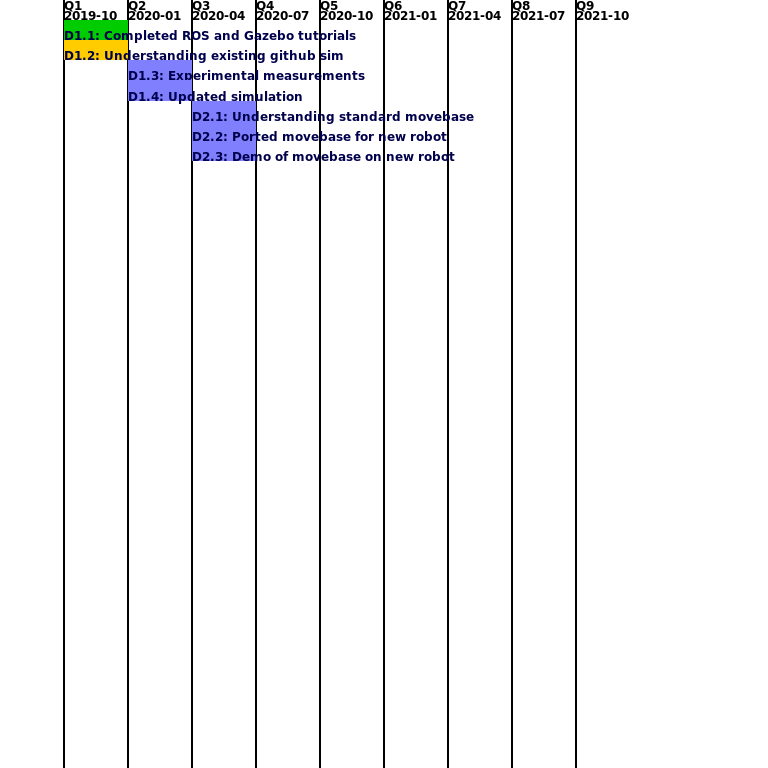
\includegraphics[width=16cm]{gantt.png}

\newpage

\section{Deliverables}

\subsection*{Deliverable D1.1: Completed ROS and Gazebo tutorials}

Start quarter: Q1 (2019-10-01) 
 
 End Quarter: Q2 (2020-01-01) 

 Leader: CHURCHILL

  Status: DONE 

 \subsubsection*{Description of work}

Demonstrate to supervisor an understanding of the complete ROS and Gazebo tutorials by running and talking through code for their final tutorials containing all taught concepts.

\subsubsection*{Associated risks:}

None

\subsubsection*{Depends on deliverables:}

None



\subsubsection*{Prerequisite for deliverables:}

D1.2: Understanding existing github sim



\subsubsection*{Resources}

\begin{tabular}{ | l | l | r | }
\hline
 Category & Partner & Cost \\ 
 \hline
 MATERIALS & LINCOLN &  2,050.00 \\ 
\hline
 \end{tabular}

Total deliverable cost:  2,050.00

\subsubsection*{Per-item costs}

\begin{tabular}{ | l | c | c | r | c | }
\hline
 Item & Partner & Category & Cost \\ 
 \hline
 Laptop PC & LINCOLN & MATERIALS & 2,000.00 FORECAST\\ 
Coffee (to enhance programming) & LINCOLN & MATERIALS & 50.00 FORECAST\\ 
\hline
 \end{tabular}

\newpage\subsection*{Deliverable D1.2: Understanding existing github sim}

Start quarter: Q1 (2019-10-01) 
 
 End Quarter: Q2 (2020-01-01) 

 Leader: CHURCHILL

  Status: INPROGRESS 

 \subsubsection*{Description of work}

Demonstrate to supervisor understanding of the existing Lincoln podcar simulation as currently on github, by running and talking through modifed version which makes the physics more realistic through modified guessed new parameters.

\subsubsection*{Associated risks:}

R2: Software learning

\subsubsection*{Depends on deliverables:}

D1.1: Understanding existing github sim



\subsubsection*{Prerequisite for deliverables:}

D1.3: Experimental measurements



\subsubsection*{Resources}

\begin{tabular}{ | l | l | r | }
\hline
 Category & Partner & Cost \\ 
 \hline
 \hline
 \end{tabular}

Total deliverable cost:  0.00

\subsubsection*{Per-item costs}

\begin{tabular}{ | l | c | c | r | c | }
\hline
 Item & Partner & Category & Cost \\ 
 \hline
 \hline
 \end{tabular}

\newpage\subsection*{Deliverable D1.3: Experimental measurements}

Start quarter: Q2 (2020-01-01) 
 
 End Quarter: Q3 (2020-04-01) 

 Leader: CHURCHILL

  Status: WAITING 

 \subsubsection*{Description of work}

Demonstrate to supervisor the accuracy of new parameters needed for the sim collected experimentally from the real robot. Likely to requrise design of suitable experiments to measure as well as some theory to understand what is needed. 

\subsubsection*{Associated risks:}

R1: Physical robots

\subsubsection*{Depends on deliverables:}

D1.2: Experimental measurements



\subsubsection*{Prerequisite for deliverables:}

D1.4: Updated simulation



\subsubsection*{Resources}

\begin{tabular}{ | l | l | r | }
\hline
 Category & Partner & Cost \\ 
 \hline
 CAPEX & LINCOLN &  200.00 \\ 
\hline
 \end{tabular}

Total deliverable cost:  200.00

\subsubsection*{Per-item costs}

\begin{tabular}{ | l | c | c | r | c | }
\hline
 Item & Partner & Category & Cost \\ 
 \hline
 Usage of physical robot & LINCOLN & CAPEX & 200.00 FORECAST\\ 
\hline
 \end{tabular}

\newpage\subsection*{Deliverable D1.4: Updated simulation}

Start quarter: Q2 (2020-01-01) 
 
 End Quarter: Q3 (2020-04-01) 

 Leader: CHURCHILL

  Status: WAITING 

 \subsubsection*{Description of work}

Design and demonstrate experiments proving that the updated simulation is accurace, eg. comparing outcomes of givign the same motion commands to the real and simulated robot. Comparisons are especially important if we want to publish this work, as they are empirical results.

\subsubsection*{Associated risks:}

None

\subsubsection*{Depends on deliverables:}

D1.3: Updated simulation



\subsubsection*{Prerequisite for deliverables:}

D2.2: Ported movebase for new robot



\subsubsection*{Resources}

\begin{tabular}{ | l | l | r | }
\hline
 Category & Partner & Cost \\ 
 \hline
 \hline
 \end{tabular}

Total deliverable cost:  0.00

\subsubsection*{Per-item costs}

\begin{tabular}{ | l | c | c | r | c | }
\hline
 Item & Partner & Category & Cost \\ 
 \hline
 \hline
 \end{tabular}

\newpage\subsection*{Deliverable D2.1: Understanding standard movebase }

Start quarter: Q3 (2020-04-01) 
 
 End Quarter: Q4 (2020-07-01) 

 Leader: CHURCHILL

  Status: WAITING 

 \subsubsection*{Description of work}

Demonstrate to supervisor running code showing understanding of standard movebase setup, eg by starting with the Clearpath Huskey simulation setup available online and modifyign some parameters based on guesswork to make it more like our robot.

\subsubsection*{Associated risks:}

R2: Software learning

\subsubsection*{Depends on deliverables:}

None



\subsubsection*{Prerequisite for deliverables:}

D2.2: Ported movebase for new robot



\subsubsection*{Resources}

\begin{tabular}{ | l | l | r | }
\hline
 Category & Partner & Cost \\ 
 \hline
 \hline
 \end{tabular}

Total deliverable cost:  0.00

\subsubsection*{Per-item costs}

\begin{tabular}{ | l | c | c | r | c | }
\hline
 Item & Partner & Category & Cost \\ 
 \hline
 \hline
 \end{tabular}

\newpage\subsection*{Deliverable D2.2: Ported movebase for new robot}

Start quarter: Q3 (2020-04-01) 
 
 End Quarter: Q4 (2020-07-01) 

 Leader: CHURCHILL

  Status: WAITING 

 \subsubsection*{Description of work}

Demonstrate ported of movebase running on the new simulated robot.

\subsubsection*{Associated risks:}

R3: Running out of time

\subsubsection*{Depends on deliverables:}

D2.1: Ported movebase for new robot

D1.4: Ported movebase for new robot



\subsubsection*{Prerequisite for deliverables:}

D2.3: Demo of movebase on new robot



\subsubsection*{Resources}

\begin{tabular}{ | l | l | r | }
\hline
 Category & Partner & Cost \\ 
 \hline
 \hline
 \end{tabular}

Total deliverable cost:  0.00

\subsubsection*{Per-item costs}

\begin{tabular}{ | l | c | c | r | c | }
\hline
 Item & Partner & Category & Cost \\ 
 \hline
 \hline
 \end{tabular}

\newpage\subsection*{Deliverable D2.3: Demo of movebase on new robot}

Start quarter: Q3 (2020-04-01) 
 
 End Quarter: Q4 (2020-07-01) 

 Leader: CHURCHILL

  Status: WAITING 

 \subsubsection*{Description of work}

Demo of movebase on new physicical robot (optional)

\subsubsection*{Associated risks:}

R1: Physical robots

\subsubsection*{Depends on deliverables:}

D2.2: Demo of movebase on new robot



\subsubsection*{Prerequisite for deliverables:}

None



\subsubsection*{Resources}

\begin{tabular}{ | l | l | r | }
\hline
 Category & Partner & Cost \\ 
 \hline
 CAPEX & LINCOLN &  200.00 \\ 
\hline
 \end{tabular}

Total deliverable cost:  200.00

\subsubsection*{Per-item costs}

\begin{tabular}{ | l | c | c | r | c | }
\hline
 Item & Partner & Category & Cost \\ 
 \hline
 Usage of physical robot & LINCOLN & CAPEX & 200.00 FORECAST\\ 
\hline
 \end{tabular}

\newpage\section{Spend profiles}

\subsection{Spend profile for partner LINCOLN}

\begin{tabular}{|r|r|r|r|r|r|r|r|r|}\hline
 X & 1 & 2 & 3 & 4 & 5 & 6 & 7 & 8  \tabularnewline
\hline
\hline
 MATERIALS & 2,050.00 & 0.00 & 0.00 & 0.00 & 0.00 & 0.00 & 0.00 & 0.00 \tabularnewline
\hline
 LABOUR & 0.00 & 0.00 & 0.00 & 0.00 & 0.00 & 0.00 & 0.00 & 0.00 \tabularnewline
\hline
 CAPEX & 0.00 & 200.00 & 200.00 & 0.00 & 0.00 & 0.00 & 0.00 & 0.00 \tabularnewline
\hline
 TRAVEL & 0.00 & 0.00 & 0.00 & 0.00 & 0.00 & 0.00 & 0.00 & 0.00 \tabularnewline
\hline
 OTHER & 0.00 & 0.00 & 0.00 & 0.00 & 0.00 & 0.00 & 0.00 & 0.00 \tabularnewline
\hline
 OVERHEADS & 0.00 & 0.00 & 0.00 & 0.00 & 0.00 & 0.00 & 0.00 & 0.00 \tabularnewline
\hline
 SUBCON & 0.00 & 0.00 & 0.00 & 0.00 & 0.00 & 0.00 & 0.00 & 0.00 \tabularnewline
\hline \end{tabular}\newpage

\section{Risk register}

\subsection*{Risk R1: Physical robots}

The phyhsical robot might not be available if needed for active Lincoln research projects, or it may be broken or being upgraded.

Category: MANAGEMENT

Treatment: MITIGATE

 The project is designed to promise only simulated results. It would be nice to demo on the real robot but this is strictly optional for delivery.

Impact Pre-Mitigation: 5

Probability Pre-Mitigation: 5

Score Pre-Mitigation: 25

Impact Post-Mitigation: 1

Probability Post-Mitigation: 5

Score Post-Mitigation: 5

Owner: CHURCHILL

Associated deliverables: D2.3 D1.3 

\subsection*{Risk R2: Software learning}

The project is based on real Lincoln research, it is not a greenfield project. As such there is a lot of existing code than needs to be understood before new development can begin. It will take time effort to get up to speed with the existing code base. This includes both open source ROS libraries such as movebase, and Lincoln's own simulation and control code as in the podcar github stack. There is a risk that a student will not be smart enough to get up to speed with all of this and still have time to make their own contribution.

Category: TECHNICAL

Treatment: MITIGATE

 The student is one of the top in the year group and has a proven track record of delivering advnaced projects from my second year group project, which scored a perfect mark of 100.  The current project should not be attempted by weaker students.

Impact Pre-Mitigation: 5

Probability Pre-Mitigation: 5

Score Pre-Mitigation: 25

Impact Post-Mitigation: 1

Probability Post-Mitigation: 1

Score Post-Mitigation: 1

Owner: CHURCHILL

Associated deliverables: D1.2 D2.1 

\subsection*{Risk R3: Running out of time}

The projcet requrires the simulation to be working before movebase can be ported. If simulation is late due to unforseen difficulty then movebase might not be delivered.

Category: TECHNICAL

Treatment: MITIGATE

 This is an inherent risk in the structure of the project. A lower-scoring project report could be submitted describing only the simulation aspects in the worst case.  Supervisor is knowledgable in the specifics of robotics research and may be able to assist to unblock technical problems to speed up simulation work if required.

Impact Pre-Mitigation: 3

Probability Pre-Mitigation: 3

Score Pre-Mitigation: 9

Impact Post-Mitigation: 2

Probability Post-Mitigation: 2

Score Post-Mitigation: 4

Owner: CHURCHILL

Associated deliverables: D2.2 

\end{document}